\documentclass[10pt,onecolumn,letterpaper]{article}

\usepackage{report}
\usepackage{times}
\usepackage{epsfig} % You can comment this out if you use pdflatex and PDF figures
\usepackage{graphicx}
\usepackage{amsmath}
\usepackage{amssymb}
\usepackage{float}
\floatstyle{plaintop}
\restylefloat{figure}
% Include other packages here, before hyperref.

% If you comment hyperref and then uncomment it, you should delete
% egpaper.aux before re-running latex.  (Or just hit 'q' on the first latex
% run, let it finish, and you should be clear).
\usepackage[pagebackref=true,breaklinks=true,letterpaper=true,colorlinks,bookmarks=false]{hyperref}


%%\reportfinalcopy % *** Uncomment this line for the final submission

\def\reportPaperID{002} % *** Enter the Project Paper ID here
\def\httilde{\mbox{\tt\raisebox{-.5ex}{\symbol{126}}}}

% Pages are numbered in submission mode, and unnumbered in camera-ready
\ifreportfinal\pagestyle{empty}\fi
\begin{document}

%%%%%%%%% TITLE
\title{\LaTeX\ Mini Project 3}

\author{Sachin Srivastava\\
Rutgers Univeristy\\
{\tt\small sachin.srivastava@rutgers.edu}
}


\maketitle
% \thispagestyle{empty}


%%%%%%%%% BODY TEXT
\section{Problem 1}
The python scripts are attached. The bias and variance estimate are as follows:\\
KNN\\
Bias: 0.0333333333333\\
Variance: 0.004\\
\\
Naive Bayes\\
Bias:0.04\\
Variance: 0.00133333333333\\
\\
As we can clearly see. The Bias for Naive Bayes is more compared to KNN, while the variance of KNN is more than Naive Bayes.
\section{Problem 2}
Since, $\theta$ is 0.5 for all class. We have $p(x_1)=p(x_1|y=c)$ for all c and $x_1$ and y are independent random variables. As consequences we get\\
i)   $p(y|x_1,x_2) = p(y|x_2)$\\
ii)  $p(y|x_1) = p(y)$\\
iii) $p(y|x_2)$\\
$$
p(x_2) = \sum_{c=1}^3 p(y=c)p(x_2|y=c)
=\frac{1}{\sqrt{2\pi}}(\frac{\exp^\frac{-(x_2+1)^2}{2}}{2} + \frac{\exp^\frac{-(x_2)^2}{2}}{4} + \frac{\exp^\frac{-(x_2-1)^2}{2}}{4} )
$$
Thus, $p(y|x_2)=\frac{p(x_2|y)p(y)}{p(x_2)}$, with $p(x_2|y) = \frac{1}{2\pi}\exp^\frac{(x_2-\mu_y)^2}{2}$\\
($\mu_y$ depends on what values y takes) and $p(x_2)$ as above.


\section{Problem 3}
Since $log \frac{p(y=1|x)}{p(y=1|x)} =0$, then $log p(x|y = 1) + log p(y = 1) = log(p(x|y = 0) + log P(y = 0)$ and since the conditional densities $p(x|y)$ are Gaussians the formula is equivalent to:\\
$$
(x - \mu_1)^T\sum_1^{-1}(x-\mu_1)+ log |\sum_1| - 2 log P(y = 1) $$
$$
= (x - \mu_0)^T\sum_0^{-1}(x - \mu_0) + log |\sum_0| - 2 log P(y = 0)
$$
and since $\sum_1 = k\sum_0$, the above formula is a quadratic formula with the main term being $(k -1)x^T\sum_0^{-1}$ which means that the decision boundary is an ellipse.

\section{Problem 4}
For a fixed $x_i$, $y_i$ are i.i.d random variables with $y_i ~ N(w_1x_i +w_0, \sigma^2)$. So the
probability distribution of $y_1$, $y_2$, ... is defined by:\\
$$f(y_1, ..., y_n|w_1,w_0) = \Pi_{i=1}^nf(y_i|w_1,w_0)$$\\
$$= \Pi_{i=1}^n\frac{1}{(2\sigma^2)^{\frac{n}{2}}} \exp^\frac{-(y_i-w_1x_i-w_0)^2}{2\sigma^2}$$
$$= \frac{1}{(2\sigma^2)^{\frac{n}{2}}} \exp^{-\frac{1}{(2\sigma^2)^{\frac{n}{2}}}\sum_{i=1}^n{(y_i-w_1x_i-w_0)^2}}$$

To get the MLE estimates of $w_1$ and $w_0$ we will set $\frac{\partial f}{\partial w_1} = 0$ and $\frac{\partial f}{\partial w_0} = 0$
which gives us the equations:\\
$$
\sum_{i=1}^nx_i(y_i-w_1x_i-w_0)=0
$$
$$
\sum_{i=1}^n(y_i-w_1x_i-w_0)=0
$$
Solving the second equation for $w_0$ yields $w_0 = y - w_1x$ and replacing $w_0$ in the first equation we can get:\\
$$
\sum_{i=1}^n(x_i-\bar{x}+\bar{x})(y_i-w_1x_i-\bar{y}+w_1\bar{x})=0
$$

which gives \\
$$
w_1 = \frac{ \sum_{i=1}^n(x_i-\bar{x})(y_i-\bar{y})}{\sum_{i=1}^n(x_i-\bar{x})}
$$

\section{Problem 5}
i) When  the number of learning observation is small the estimate $\mu\sum^*$ become inexact and result in the classification error of observation vectors which do not participate in the design of the classification rule.\\

ii) In the two class case we will have $p(y=1|x,\theta)= \sigma(\beta_1-\beta_0)^Tx+(\gamma_1-\gamma_0)$

In this case, The decision boundary will get shifted depending on the priors. \\

iii) It will not be a problem in that case as the co-variance matrix has the correct estimate.\\
\\\\\\\\\\\\\\\\\\\\\\\\\\\\\\\\\\\\\\\
\section{Problem 6}

\begin{figure}[ht!]
\centering
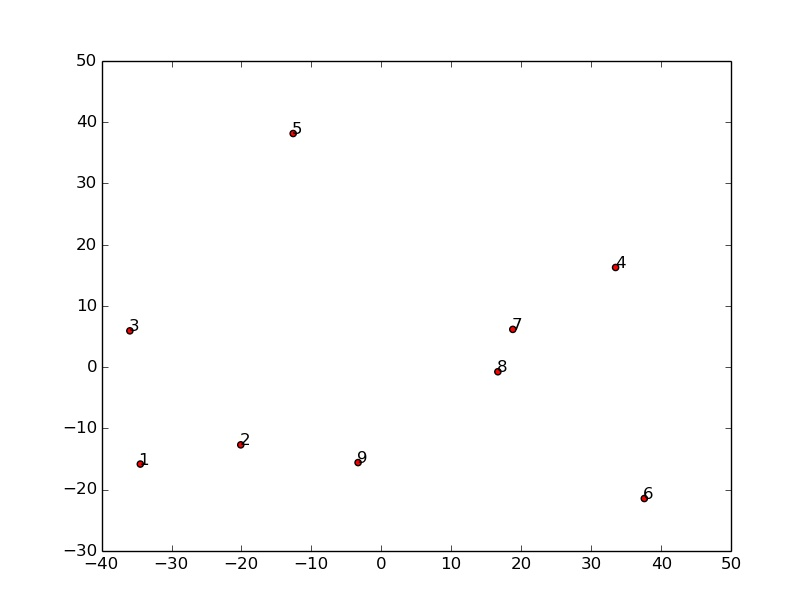
\includegraphics[width=120mm]{figure_1.jpg}
\caption{PCA for points 1-9 \label{overflow}}
\end{figure}

\begin{figure}[ht!]
\centering
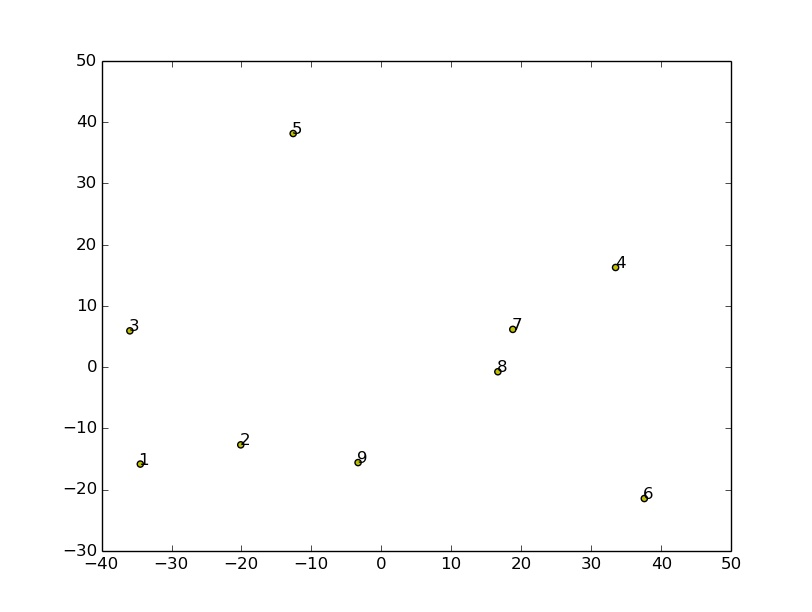
\includegraphics[width=120mm]{figure_2.jpg}
\caption{PPCA for points 1-9: The points for PPCA are same as the for PCA. \label{overflow}}
\end{figure}

\begin{figure}[ht!]
\centering
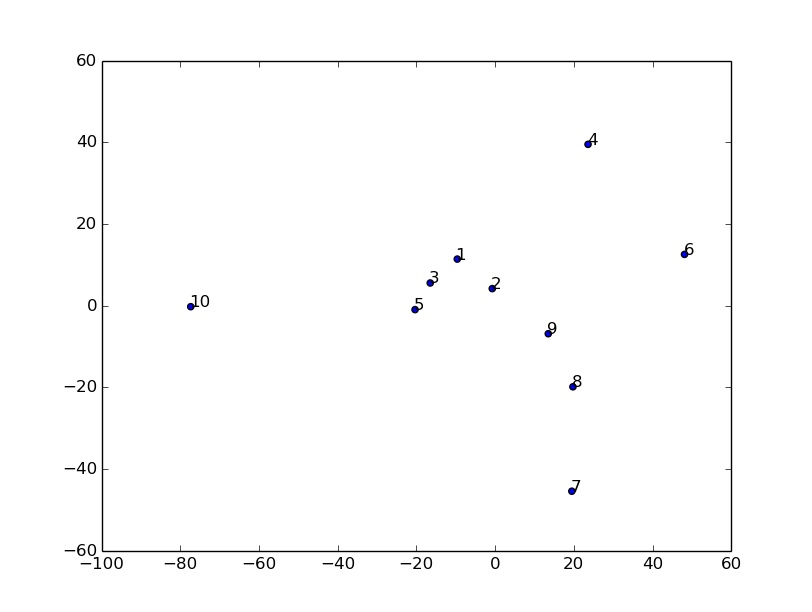
\includegraphics[width=120mm]{figure_3.jpg}
\caption{PCA for points 1-9: Above is the result after adding dummy point q to the data. The top 3 closest points are 5, 3, 1. While 3 and 1 are expected to be closer but we are also getting point 5 as a close point. \label{overflow}}
\end{figure}

\begin{figure}[ht!]
\centering
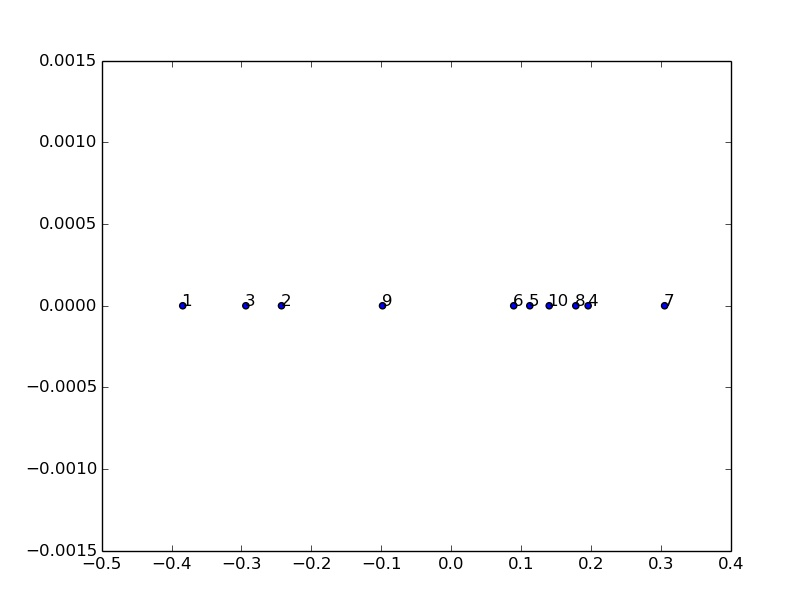
\includegraphics[width=120mm]{figure_4.jpg}
\caption{PCA for points 1-9 : Using Fishers LDA the top 3 closest points are 5, 8 and 4. These are different from the points using PCA. Only point 5 is common.\label{overflow}}
\end{figure}

\end{document}
